% "{'classe':('PSI','MP'),'chapitre':'slci_revisions','type':('td'),'titre':'Contrôle d\\'une machine de forage', 'source':'Concours CCINP 2023 - MP','comp':[],'corrige':True}"
%\setchapterimage{bandeau}
\chapter*{TD \arabic{cptTD} \\ 
Contrôle d'une machine de forage -- 
\ifprof Corrigé \else Sujet \fi}
\addcontentsline{toc}{section}{TD \arabic{cptTD} :
Contrôle d'une machine de forage -- 
\ifprof Corrigé \else Sujet \fi}

\iflivret \stepcounter{cptTD} \else
\ifprof  \stepcounter{cptTD} \else \fi
\fi

\setcounter{question}{0}
\marginnote{D'après Concours CCINP 2023 -- MP.}
%\marginnote[1cm]{
%\UPSTIcompetence[2]{C1-02}
%\UPSTIcompetence[2]{C2-04}}




\ifprof
\else
On travaille avec le schéma-bloc simplifié de la figure \ref{Cy_02_Ch_04_TD_03_fig_12} où $K_0$ est un gain d’adaptation fixe. 


\begin{figure}[!h]
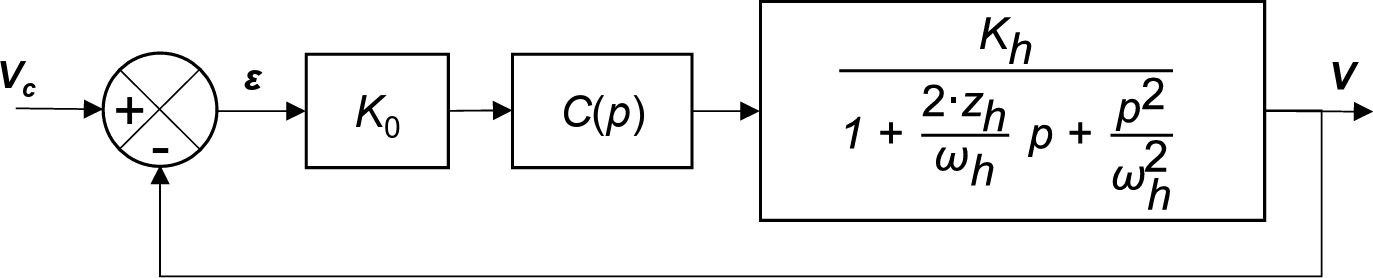
\includegraphics[width=.7\linewidth]{fig_12}
\caption{Schéma-bloc de l’asservissement en vitesse simplifié \label{Cy_02_Ch_04_TD_03_fig_12}}
\end{figure}

 On prend dans un premier temps un correcteur $C(p)$ proportionnel : $C(p) = K_p$. 
 \fi
 
%Q 25
\question{Exprimer la fonction de transfert en boucle ouverte $\indice{G}{BO}(p)=\dfrac{V(p)}{\varepsilon(p)}$.}
\ifprof
\begin{corrige}

$\indice{G}{BO}(p) = K_0 C(p) \ordredeuxopt{K_h}{z_h}{\omega_h}$
 
\end{corrige}

\else
\fi


\begin{marginfigure}
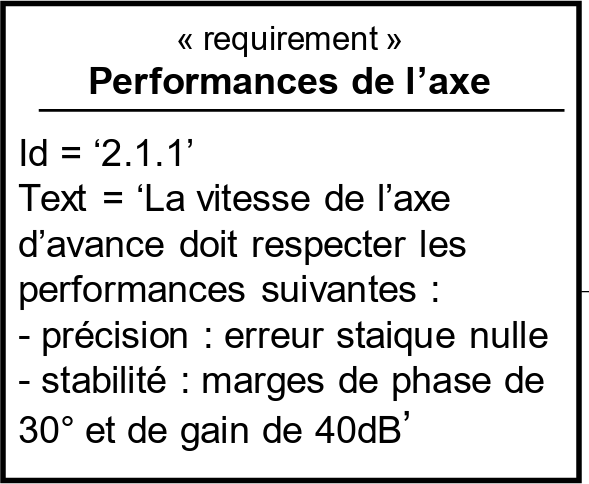
\includegraphics[width=\linewidth]{req}
%\caption{ Schéma-bloc de l’asservissement en vitesse simplifié \label{Cy_02_Ch_04_TD_03_fig_12}}
\end{marginfigure}

%Q26. 
\question{Avec un correcteur proportionnel, peut-on satisfaire l’exigence de précision de vitesse 
indiquée à l’exigence 2.1.1. ? Justifier.}
\ifprof
\begin{corrige}
Pour un erreur statique nulle, il faut oblogatoirement un intégrateur dans la boucle ouverte, ce qui n'est pas le cas. 
\end{corrige}
\else
\fi

 
On utilise dans un second temps un correcteur proportionnel intégral : $C(p)=K_P\left( 1+\dfrac{1}{T_i p}\right)$.
 
%Q27. 
\question{L’exigence de précision sur la vitesse est-elle satisfaite ? Justifier. }
\ifprof
\begin{corrige}
$C(p)=K_P\left( 1+\dfrac{1}{T_i p}\right)$ $= K_P\dfrac{T_i p + 1}{T_i p}$. 
La FTBO est maintenant de classe 1. L'erreur statique est donc nulle.
\end{corrige}
\else
\fi

 Ce correcteur est initialement réglé avec les valeurs suivantes : $K_p = 1$ et $T_i = \SI{10}{s}$. 
 
%Q28. 
\question{Tracer les diagrammes de Bode asymptotique et réel de ce correcteur. Détailler 
les constructions. }
\ifprof
\begin{corrige}

On a $\dfrac{K_p}{T_i} = 0,1$
\begin{itemize}
\item Quand $\omega$ tend vers 0, le gain a une pente de \SI{-20}{dB/decade} et la phase tend vers \SI{-90}{\degres}.
\item Quand $\omega$ tend vers $+\infty$, le gain a une pente de \SI{0}{dB/decade} et tend vers $20\log K_p = 0$  et la phase tend vers \SI{0}{\degres}.
\item Le changement de pente se passe à 1/10 \si{rad/s}.
\end{itemize}

\begin{center}
\begin{tikzpicture}[xscale=15/6]
\tikzset{
semilog lines/.style={thin, bleuxp}, 
semilog lines 2/.style={semilog lines,bleuxpc},
semilog half lines/.style={semilog lines 2,dotted },
semilog label x/.style={semilog lines,below,font=\tiny,black},
semilog label y/.style={semilog lines,right,font=\tiny,black}
}
\begin{scope}[yscale=3/140]
\OrdBode{20}
\semilog{-3}{1}{-20}{60}
\BodeAmp[orangexp,thick,samples=150]{-3:1}{-\POAmpAsymp{1}{10}+\IntAmp{1}+\KAmp{0.1}}
\BodeAmp[orangexp,ultra thick,samples=150]{-3:1}{-\POAmp{1}{10}+\IntAmp{1}+\KAmp{0.1}}

%\draw (-1.5,28) node {\footnotesize $20\log K$};
%\draw (1.1,10) node {\footnotesize $-$40 dB/d\'ecade};
%\draw [dashed,ultra thick,bleuxp] (-.08,-60) -- (-.08,25);
%\draw (-.08,-60)  node {\Huge $\cdot$} node [above right]{\footnotesize $\omega_0$};
\end{scope}
\begin{scope}[yshift=-1cm,yscale=1/90]
\UniteDegre
\OrdBode{45}
\semilog{-3}{1}{-180}{0}
%\BodeArg[orangexp,thin,samples=150]{1:5}{\POArgAsymp{1773}{0.000794}+\IntAmp{1}}
\BodeArg[orangexp,thick,samples=150]{-3:1}{-\POArgAsymp{1}{10}+\IntArg{1}}
\BodeArg[orangexp,ultra thick,samples=190]{-3:1}{-\POArg{1}{10}+\IntArg{1}}

%\BodeArg[orangexp,samples=100,thin]{-2:2}{\SOArg{10}{0.2}{.9}}
%\BodeArg[orangexp,ultra thick]{-2:2}{\SOArg{10}{0.2}{.9}}
\end{scope}
\end{tikzpicture}
\end{center}


\end{corrige}
\else
\fi


\ifprof
\else
\begin{figure}[!h]
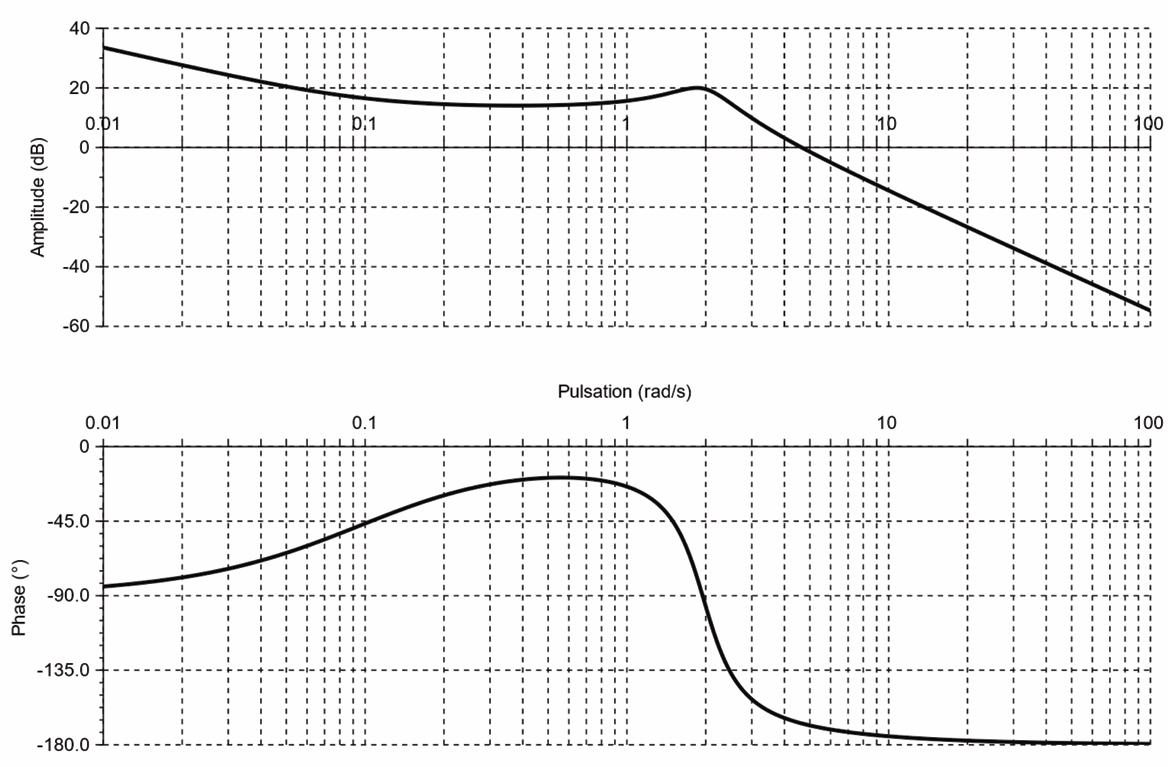
\includegraphics[width=\linewidth]{dr_03}
%\caption{ Schéma-bloc de l’asservissement en vitesse simplifié \label{Cy_02_Ch_04_TD_03_fig_12}}
\end{figure}

 
Pour le réglage de la question précédente, on donne le diagramme de Bode de la fonction de 
transfert en boucle ouverte ainsi corrigée sur le DR3. 
\fi

% Q29. 
\question{Affiner le réglage du correcteur (sans modifier la valeur de $T_i$) en proposant une valeur de $K_p$ permettant de garantir la marge de phase spécifiée dans l’exigence 2.1.1. }%On répondra à cette question sur la figure précente.}
\ifprof
\begin{corrige}
Pour avoir une marge de phase de 30\degres, il faut que le gain soit nul quand la phase est de $-150\degres$. Dans l'état actuel le gain est de \SI{10}{dB}. Il faut donc $20\log K_P = -10$ soit $K_P = 0,31$.
\end{corrige}
\else
\fi
 
 
\ifprof
\else
Enfin, on souhaite valider ou invalider l’hypothèse faite en début de cette sous-partie concernant la 
non-influence de l’amortisseur sur les performances d’asservissement en vitesse d’avance de la 
table de forage. Les diagrammes de Bode de la figure suivante, 
illustrent la fonction de transfert en boucle ouverte corrigée sans (en train plein) et avec amortisseur 
(en pointillés). 
 
 
\begin{figure}[!h]
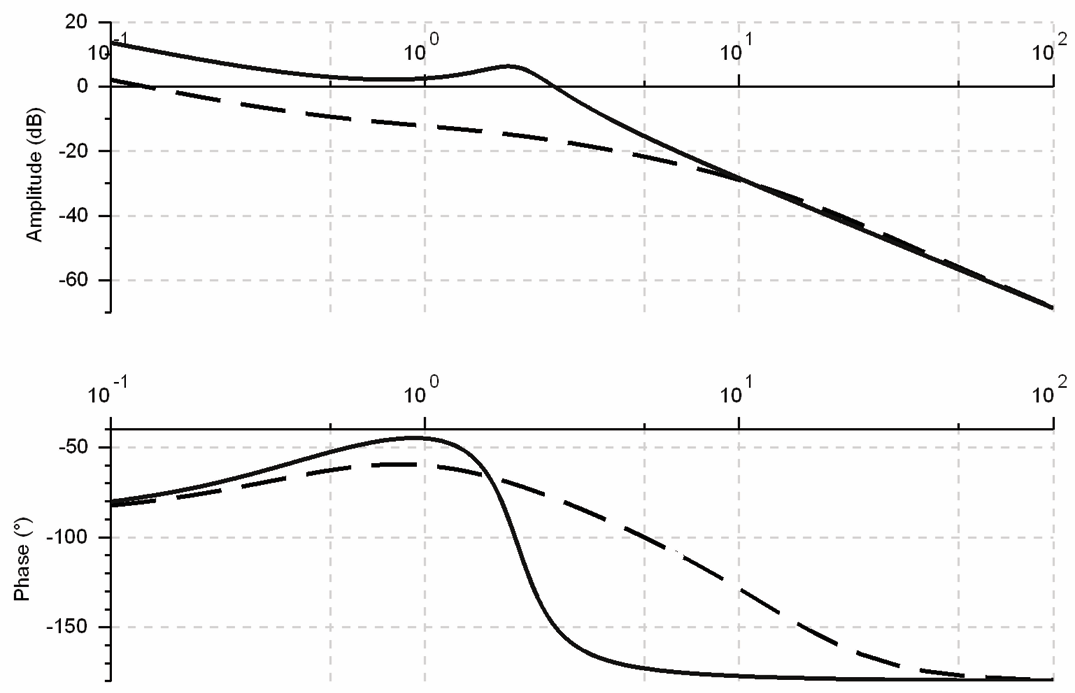
\includegraphics[width=\linewidth]{dr_04}
%\caption{ Schéma-bloc de l’asservissement en vitesse simplifié \label{Cy_02_Ch_04_TD_03_fig_12}}
\end{figure}
\fi
 
\ifprof
\else
\begin{marginfigure}
\centering

\includegraphics[width=3cm]{Cy_02_Ch_04_TD_03_qr}
\end{marginfigure}
\fi

%Q30. 
\question{Sur quelle(s) performance(s) la présence de l’amortisseur peut-elle influer ? Justifier que le correcteur choisi permet de répondre aux exigences 2.1.1 en présence de l'amortisseur.}
\ifprof
\begin{corrige}
L'amortisseur améliore la stabilité car la marge de phase est plus grande. En revanche, la bande passante à \SI{0}{dB} étant plus petite, le système est donc moins rapide.
\end{corrige}
\else
\fi




